%%%%%%%%%%%%%%%%%%%%%%%%%%%%%%%%%%%%%%%%
%%%                                  %%%
%%%  The paper about the G-Prop      %%%
%%%              NPL                 %%%
%%%%%%%%%%%%%%%%%%%%%%%%%%%%%%%%%%%%%%%%
\documentclass{llncs}
\usepackage{graphics}

\def\CC{{C\hspace{-.05em}\raisebox{.4ex}{\tiny\bf ++}}~}
\addtolength{\textfloatsep}{-0.5cm}
\addtolength{\intextsep}{-0.5cm}


%%%%%%%%%%%%%%%% Titulo %%%%%%%%%%%%%%%
\title{Evolving Multilayer Perceptrons}
\author {P.A. Castillo \inst{1}, J. Carpio \inst{1}, J.J. Merelo \inst{1}, A. Prieto \inst{1}, V. Rivas \inst{2} and G. Romero \inst{1}}
\institute{Department of Architecture and Computer Technology \\
           University of Granada \\
           Campus de Fuentenueva \\
           E. 18071 Granada (Spain) \\
\and       Departament of Computer Science  \\
           University of Ja\'{e}n\\
           Avda. Madrid, 35 \\
           E. 23071 Ja\'{e}n (Spain) \\
~\\
           Phone: {\tt +34 958 243162}\ \ \ \ \ Fax: {\tt +34 958 248993}
~\\
           e-mail: {\tt todos@geneura.ugr.es}\ \ \ \ \ URL: {\tt http://geneura.ugr.es} }

\date{} 

\begin{document}
\maketitle
 
 
\begin{abstract} 
This paper proposes a new version of a method (G-Prop, genetic backpropagation) that attempts to solve the problem of finding appropriate initial weights and learning parameters for a single hidden layer Multilayer Perceptron (MLP) by combining an evolutionary algorithm (EA) and backpropagation (BP). The EA selects the MLP initial weights, the learning rate and changes the number of neurons in the hidden layer through the application of specific genetic operators, one of which is BP training.
The EA works on the initial weights and structure of the MLP, which is then trained using QuickProp; thus G-Prop combines the advantages of the global search performed by the EA over the MLP parameter space and the local search of the BP algorithm. 
The application of the G-Prop algorithm to several real-world and benchmark problems shows that MLPs evolved using G-Prop are smaller and achieve a higher level of generalization than other perceptron training algorithms, such as QuickPropagation or RPROP, and other evolutive algorithms. It also shows some improvement over previous versions of the algorithm. \\

\textbf{Keywords}: Evolutionary Algorithms, Generalization, Learning, Neural Networks, Optimization
\end{abstract} 
 

%%%%%%%%%%%%%%%% Introduction %%%%%%%%%%%%%%%

\cleardoublepage

\section{Introduction and State of the Art}
\label{sec:intro}

The use of artificial neural networks (ANNs) requires establishing the structure in layers and connections between them, the parameters (such as initial weights) and a set of learning constants. 
The training mechanism is usually an iterative gradient descent algorithm, designed to minimize, step by step, the difference between the actual output vector of the network and the desired output vector, such as BP in its different versions (like, for instance QuickProp, QP, by \cite{FahlmanQP} and RPROP by Riedmiller and Braun \cite{Riedmiller93}). Some evolutionary approaches \cite{competitiveNNGA,Castillo2,Yao98,Yao98b,Miller} are also used.
However, this method, successful as it is in many fields, does encounter certain difficulties in practice:
1) the convergence tends to be extremely slow; 2) convergence to the global optimum is not guaranteed; 3) learning constants and other parameters must be arrived at heuristically.

These latter two problems, premature convergence and parameter setting, have been approached using several optimization procedures, which can be divided into two groups: Incremental / Decremental (see \cite{Alpaydim}, by Alpaydim et al. for a review) or genetic algorithms, which are reviewed for instance in \cite{balakrishnan95:EDNA}.

\begin{itemize}
      \item \emph{Incremental algorithms}, are based on adding hidden neurons to a network of minimum size until the required precision is reached. These methods start with few hidden neurons and increase their number until the error is sufficiently small. This approach is used in the \emph{Cascade Correlation Algorithm} (by Fahlman and Lebi\`{e}re \cite{FahlmanCASCOR}), the \emph{Tiling and Perceptron Cascade Algorithm} (by Parekh et al. in \cite{Parekh}) and in the method proposed by Rathbun et al. \cite{Rathbun}.

\noindent One problem of these methods is that once the hidden neurons have been added they cannot be suppressed to reduce the size (the redundant information stored in the weights is never eliminated) and huge ANNs are usually obtained. Furthermore, since the weights of existing neurons are frozen, the added ones are usually inefficient feature detectors, so the algorithm has to add even more units to improve the results obtained. In general, as J. Hwang et al. showed in \cite{Hwang}, adding new units leads to overfitting.

      \item \emph{Decremental algorithms}, also called pruning methods, are based on taking a network with an initially high number of connections, and then eliminating them one by one or setting them to zero, to obtain a smaller network but with the same (or better) classification ability.
These algorithms work by searching for redundant noncontributing or duplicate nodes.
After pruning, the ANN must usually be re-trained.
This approach is used by Jasic et al. in \cite{Jasic}, Pelillo et al. in \cite{Pelillo}, in the \emph{Optimal Brain Damage Algorithm} (by Le Cun et al. \cite{LeCun}) and in the \emph{Optimal Brain Surgeon Algorithm} (by Hassibi et al. \cite{Hassibi}).

\noindent The problem with these methods is that they start with excessively large networks, which slows down training. However, depending on the selection criteria used to select the neurons to be pruned, it is possible to obtain a good solution, if the units to eliminate and the elimination order are guessed correctly.
\end{itemize}

In any case, both decremental and incremental algorithms are gradient descent optimization methods, so they suffer the problem that they may reach the local minimum closest to the search space point where the method began.

\bigskip

\emph{Evolutionary neural networks} provide an alternative for the task of controlling the complexity by adjusting the number of weights of the ANN, which is an example of a \emph{hybrid approach} of a GA and BP to train an ANN. 
GAs can be applied to design ANNs in several ways \cite{Yao92,Marin95}:

\begin{itemize}
      \item \emph{Search for the optimal set of weights}: some authors use a purely evolutionary approach using binary coding of weights (Topchy et al. \cite{Topchy}, Falco et al. \cite{FalcoPPSN98} and Whitley et al. \cite{Whitley93}) or Gray encoding (Schraudolph and Belew \cite{Schraudolph92}).
In other cases, as in \cite{Castillo1}, a GA and gradient descent algorithm are combined, as Keesing and Stork did in \cite{Keesing}, where they take advantage of the Baldwin effect \cite{Baldwin} to increase the rate of evolution.

\noindent The main problem with these approaches is that they concentrate on optimizing only a part of the neural net, disregarding the rest: the hidden layer size and the learning constants.


      \item \emph{Search over topology space}: some authors use a GA whose population is a set of complete ANNs, initialized with different hidden layer sizes (White et al. in \cite{White}, Yao and Liu \cite{Yao98,Yao98b} and Falco et al. \cite{Falco2}); a method to prune oversized networks is also used (Bebis et al. \cite{Bebis}).

\noindent Miller et al. \cite{Miller} propose a method in which the network connection structure is mapped onto a binary adjacency matrix called the \emph{Miller-Matrix} that describes the ANN architecture, but a problem with this approach is the matrix representation of the network. Incorrect network structure, i.e. feedback connections, and very long codes for larger networks are the result. To avoid this problem, some methods of indirect coding have been proposed, such as those of Kitano \cite{Kitano90b}, Harp et al. \cite{Harp89}, Dodd et al. \cite{Dodd91} and Gruau \cite{Gruau92}.


      \item \emph{Search for the optimal learning parameters}, including weights, having pre-established the number of neurons and the connectivity between them, as did Merelo et al. in \cite{competitiveNNGA}, for multilayer competitive learning neural nets, where a method that codifies the weights and learning parameters onto chromosomes is presented. Another example is the method presented by Petridis et al. in \cite{Petridis} where both weights and learning parameters are represented as bit strings to be evolved. Another approach that searches for the learning parameters of the net, based on Simulated Annealing, is proposed by Castillo et al. in \cite{Castillo2}.

\end{itemize}

Evolutionary neural networks are a more efficient way of searching, but they still search within a subset of all possible parameters (for instance, weights or learning constants).

The aim of this paper is to present an algorithm to tune learning parameters and to set the initial weights and hidden layer size of a MLP, based on an EA and BP. 
A method to search for the optimal set of weights, the optimal topology and learning parameters, using an EA and BP, was proposed by Castillo et al. in \cite{Castillo3}; in that case, however, the learning constant was set by hand. This new version of the method does not need any constant related to the ANN to be set by hand. It obviously needs to set the EA constants, but is robust enough to obtain good results under the default parameter settings.

In G-Prop we intend to make use of the capacities of both algorithms: the ability of EA to find a solution close to the global optimum, and the ability of the BP to tune a solution and reach the nearest local minimum by means of local search from the solution found by the EA.
Instead of using a pre-established topology, the population is initialized with different hidden layer sizes, with some specific operators designed to change them.
As genetic operators, mutation, multi-point crossover, addition, elimination and substitution of hidden units, and QP training applied as operator to the individuals of the population, are used.
Thus, the EA searches and optimizes the architecture (number of hidden units), the initial weight setting for that architecture and the learning rate for that net.
Unlike other approaches \cite{Yao98}, the maximum size of the hidden layer is not bounded in advance.


The main differences between G-Prop and other evolutionary methods of perceptron training are:
\begin{itemize}
      \item An EA is applied directly to a population of MLPs, instead of performing some codification of the network. Thus a linear or binary representation is not needed to evolve the population, which avoids possibly incorrect solutions.
      \item The EA is only used to modify the initial weights, while BP is used to train from those weights. BP can also be used as a genetic operator, which means that, while trained weights are not usually put back into the evolved MLP, if BP is used as a genetic operator, ANN trained weights remain in the population. This creates a clean division between global and local search.
      \item The hidden layer size is searched through the aplication of new GA operators: substitution, addition and elimination. These operators are developed to perform incremental (adding hidden neurons) or decremental (pruning hidden neurons) learning.
\end{itemize}

The remainder of this paper is structured as follows: Section \ref{sec:method} presents the G-Prop algorithm, followed by the architecture and genetic operators. Section \ref{sec:expe} describes the experiments and results obtained, followed by a brief conclusion in Section \ref{sec:conclus}.
 

%%%%%%%%%%%%%%%% Method %%%%%%%%%%%%%%%
\section{The evolutionary algorithm in G-Prop}
\label{sec:method}

The designed algorithm is specified in the following pseudocode:

\begin{enumerate} 
	\item Generate the initial population with random weight values and hidden layer sizes ranging uniformly distributed from 2 to a maximum of MAX (this is needed in order to have a diversity of sizes). The initial learning parameter is initialized with random values ranging from 0.01 to a maximum of 0.3.
	\item Repeat for $g$ generations:
		\begin{enumerate} 
			\item Evaluate the new individuals: train them using the training set and obtain their fitness according to the number of correct classifications on the validation set and the hidden layer size.
			\item Select the $n$ best individuals in the population, according to their fitness, and apply genetic operators to copies of them.
			\item Replace the $n$ worst individuals with the new ones.
		\end{enumerate} 
	\item Use the best individual to obtain the testing error.
\end{enumerate} 

The classification accuracy or number of hits is obtained by dividing the number of hits among the total number of examples in the testing set.
In G-Prop the \emph{fitness function} is given by the number of hits obtained when carrying out the test after training, and in the case of two individuals with identical classification error (measured as the number of elements incorrectly classified) the best is the one that has a hidden layer with fewer neurons. This implies greater speed when training and classifying and facilitates its hardware implementation. 

A \emph{steady state} \cite{Whitley} algorithm was used because it was empirically found to be faster at obtaining solutions than other selection algorithms. For each generation, the best $n$ individuals of the population, those whose fitness is highest, are chosen to mate, using the genetic operators. The offspring replace the $n$ worst individuals of the current generation.


In principle, evolved MLPs should be codified into chromosomes to be handled by the genetics operators of the EA. But G-Prop uses no binary codification; instead, the initial parameters of the network are evolved using specific genetic operators (see below), such as mutation, crossover and the substitution, addition and elimination of hidden neurons, which is made possible by the \textbf{EO} (Evolvable$|$Evolutionary Objects) library philosophy (see next section): any object with a fitness can be evolved. Moreover, this agrees with the spirit of Z. Michalewicz: $GA + DS = EP$ (GA plus Data Structures equals Evolution Programs) \cite{Michalewicz} . The genetic operators act directly on the ANN object, but only \emph{initial weights} and the \emph{learning rate} are subjected to evolution, not the weights obtained after training (a clone of the MLP is created to compute its fitness function, thus the initial weights remain unchanged in the original MLP). The ``genetic atom'' is a hidden layer neuron; most operators treat hidden layer neurons and weights to and from it as an unit.

Six genetic operators are used to change MLPs. Besides the percentage of mutation and the number of crossing points, the application priority for each operator has to be specified to indicate the number of individuals generated by each genetic operator. The tests have been done using a higher priority for mutation and the same level for the remaining operators. 
\begin{itemize}

\item The \emph{mutation} operator modifies the weights of certain neurons, at random, depending on the application rate. It is based on the algorithm presented in \cite{Kinnebrock}, which modifies the weights of the network after each epoch of network training, adding or subtracting a small random number that follows \emph{uniform} distribution with the interval $[-0.1,0.1]$.
The learning rate is modified by adding a small random number that follows \emph{uniform} distribution in the interval $[-0.05,0.05]$. This operator was used with an application probability of $40\%$, that is $40\%$ of weights are changed, which was found empirically to obtain better results than did lower probabilities.

\item The \emph{CrossOver} operator carries out the multipoint cross-over between two chromosome nets, so that two networks are obtained whose hidden layer neurons are a mixture of the hidden layer neurons of both parents: some hidden neurons along with their \emph{in} and \emph{out} connections, from each parent make one offspring and the remaining hidden neurons make the other one.
The learning rate is swapped between the two nets.

\item The \emph{Addition} operator and the following (Elimination) attempt to solve one of the main problems of BP and its variants: the difficulty in guessing the number of the hidden layer neurons. By adding hidden neurons it is not necessary to set the size of the EA search space.
This operator is intended to perform incremental learning: it starts with a small structure and increments it, if neccesary, by adding new hidden units. 
At the same time, it raises the dilemma of overfitting: small networks generalize well, but they are slow learning, whereas big networks are fast learning, but generalize badly \cite{Bellido,Bebis}. That is why it is combined with the following operator.

\item The \emph{Elimination} operator eliminates one hidden neuron at random. This operator is intended to perform decremental learning: it prunes certain nodes to obtain better results in generalization and a smaller network \cite{Jasic,Pelillo,Bebis}. Thus, to a certain extent, the networks are prevented from growing too much.

\item The \emph{Substitution} operator is applied at a low priority and replaces one hidden layer neuron at random with a new one, initialized with random weights. This operator may be considered a kind of mutation that affects only one gene.


\item The \emph{Training} operator is the main difference between the new version of G-Prop and previous versions. This operator is used to train the individual-net for a certain number of generations, using the QP algorithm, as suggested in \cite{Montana} and \cite{Yao98}. This strategy implements Lamarckism (i.e., that individuals inherit properties acquired from their parents).

\end{itemize}

The algorithm was run for a fixed number of generations.
When evaluating each individual of the population to obtain its fitness a limit of epochs was established. 
 

%%%%%%%%%%%%%%%% experiments and results %%%%%%%%%%%%%%%
\section{Experiments and results}
\label{sec:expe}

We used the \textbf{EO} library as a toolbox to develop G-Prop, due to the facility that this library offers to evolve any object with a fitness function and use anything as a genetic operator. EO is a C++ toolbox which defines interfaces for many classes of algorithms used in evolutionary computation and, at the same time, provides some examples that use those interfaces. It is available at {\sf http://geneura.ugr.es/\symbol{126}jmerelo/EO.html}. One of the objectives of using EO is to make it easier to reproduce results, which is why the source for all objects evolved with EO should also be made available, together with the articles that mention them. G-Prop is available at {\sf http://geneura.ugr.es/\symbol{126}pedro/G-Prop.htm}

First, we show the dynamics of G-Prop as an evolutionary algorithm and then compare it with other methods.
The evolution of classification error and hidden layer size during a typical run are shown in Figure  \ref{fig:graf}, usually, each of these quantities is optimized in turn: classification error is optimized first, since it is given higher priority in fitness evaluation; then, while keeping the same classification accuracy, G-Prop optimizes size. 

In the run shown in Figure \ref{fig:graf}, in generation 6, a MLP with better classification accuracy but more hidden neurons (4) is found; later on during the simulation (generation 10) a perceptron with the same accuracy but fewer hidden neurons (3) is selected as the best. And finally, at generation 18, a MLP with even fewer neurons (2) is selected as the winner.

G-Prop was run 20 times with the same parameter settings and a different random initialization for each benchmark used.

\begin{figure}[!h] 
\begin{center}
\begin{tabular}{cc}
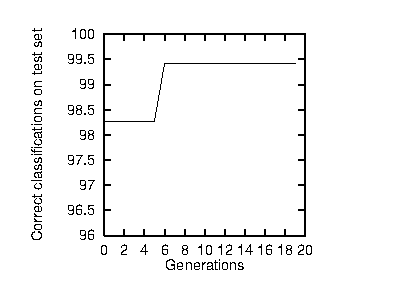
\includegraphics{hit.eps} & 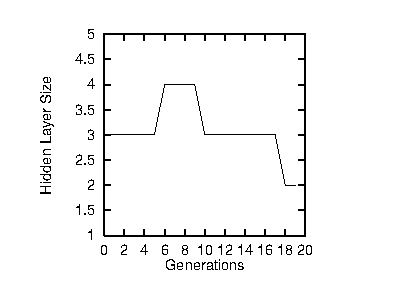
\includegraphics{size.eps} \\
a & b
\end{tabular}
\end{center}
\label{fig:graf}
\caption{\small{Evolution of the classification error of G-Prop in terms of hit percentages and hidden layer size during a typical run on the \emph{Cancer1a} set. At generation 6, a MLP with better classification accuracy but more hidden neurons (4) is found; later on during the simulation (generation 10) a perceptron with better accuracy but fewer hidden neurons (3) takes its place. And finally, at generation 18 a MLP with the same accuracy but fewer hidden neurons (2) is selected as the winner.}}
\end{figure}

The tests used to assess the accuracy of both methods must be chosen carefully, because some of them (exclusive-or problem) are not suitable for certain capacities of the BP algorithm, such as generalization \cite{FahlmanBENCHMARKS}. Our opinion, along with Prechelt \cite{Prechelt94c}, is that to test an algorithm, at least two real world problems should be used.

The tests were applied as follows: each data set was divided into three disjoint parts, for training, validating and testing. In order to obtain the fitness of an individual, the MLP is trained with the training set and its fitness is established from the classification error with the validating set. 
Once the EA is finished (when it reaches the limit of generations), the classification error with the testing set is calculated: this is the result shown.

The results which have an error greater than five times the error average are not taken into account to obtain the final results.

The {RPROP} results, quoted here come from Prechelt \cite{Prechelt94c}. 
The basic principle of {RPROP} \cite{Riedmiller93,Riedmiller94} is to eliminate the influence of the size of the partial derivative on the weight step. As a consequence, only the sign of the derivative is considered to indicate the direction of the weight update. This BP variant is one of the best at avoiding local minima (one of the problems of BP) because the magnitude of the change in the weights (the step size) is not a function of the magnitude of the gradient.

Gr\"{o}nroos \cite{MAG98} used both \emph{Cancer1a} and \emph{Glass} data sets to test an EA that used different codifications of networks (Miller, Kitano, Nolfi, Cangelosi). The results we quote here are those obtained using Kitano's coding (the best he found for all the codifications). Kitano's method \cite{Kitano90a,Kitano90b} is based on a context-free and deterministic generation grammar to encode individuals, and a genetic algorithm that uses fitness-proportional selection, elitism, single and multiple crossover and mutations.

\emph{Cancer1a.} \\
Diagnosis of breast cancer. Try to classify a tumor as either benign or malignant based on cell descriptions gathered by microscopic examination.
This dataset comes from the UCI machine learning dataset called "Wisconsin breast cancer database". It was obtained from the University of Wisconsin  Hospitals, Madison from Dr. William H. Wolberg \cite{Wolberg}.
An exhaustive report, by Prechelt, on this dataset (and others) is given in \cite{Prechelt94c}.
Each sample has 10 attributes plus the class attribute: Sample code number, Clump Thickness, Uniformity of Cell Size, Uniformity of Cell Shape, Marginal Adhesion, Single Epithelial Cell Size, Bare Nuclei, Bland Chromatin, Normal Nucleoli, Mitoses, Class (0 for benign, 1 for malignant).
The class distribution in the original set is the following: $65.5\%$ Benign and $34.5\%$ Malignant.

\emph{Glass.} \\
This problem consists of the classification of glass types, and is also taken from \cite{Prechelt94c}. The results of a chemical analysis of glass splinters (percent content of 8 different elements) plus the refractive index are used to classify the sample to be either float processed or non float processed building windows, vehicle windows, containers, tableware, or head lamps. This task is motivated by forensic needs in criminal investigation.
This dataset was created based on the glass problem dataset from the UCI repository of machine learning databases.
The data set contains 214 instances. Each sample has 9 attributes plus the class attribute: refractive index, sodium, magnesium, aluminum, silicon, potassium, calcium, barium, iron, class attribute (type of glass).

For the \emph{Cancer1a} problem the EA was executed using the parameters shown in Table \ref{table:parametros}.
\begin{table*}[!h]
\begin{center}
\begin{tabular}{|c|c|}
\hline 
Parameter & Value \\
\hline
\hline
number of generations & 20 \\
\hline
individuals in the population & 20 \\
\hline
mutation probability & 0.4 \\
\hline
crossing points & 2 \\
\hline
$\%$ of the population replaced & $50\%$ \\
\hline
inputs & 9 \\
\hline
hidden units & ranging from 2 to 20 \\
\hline
outputs & 2 \\
\hline
epochs to calculate fitness & 100 \\
\hline
initial learning coefficient & ranging from 0.01 to 0.3 \\
\hline
\end{tabular}
\end{center}
\caption{\small{List of parameters used to execute the EA on the \textbf{Cancer1a} benchmark.}}
\label{table:parametros}
\end{table*}

Yao and Liu present a method to evolve modular neural networks and the results obtained for the cancer problem in \cite{Yao98b}. While the results they present are better on classification accuracy ($0.037 \pm 0.012$), the network sizes obtained are greater ($13.1 \pm 1.2$) than those obtained using G-Prop. Moreover, we have not included Yao's results in table \ref{table:cancer} because they do not mention which set they use.

The results obtained for the first test ($\%$ of error in test), compared with those obtained by Prechelt \cite{Prechelt94c}, Castillo et al. \cite{Castillo1,Castillo2} and Gr\"{o}nroos \cite{MAG98}, are shown in Table \ref{table:cancer}.

\begin{table*}[!h]
\begin{center}
\begin{tabular}{|c||c|c|c|c|c|}
\hline 
Method & Error $\pm$ $\sigma$ & Size $\pm$ $\sigma$ (params.) &  Best Learning P. \\
\hline
\hline
G-Prop$^1$   &  1.0  $\pm$ 0.4   &  2 $\pm$ 1  (22)       & 0.124654  \\
\hline
G-Prop$^2$   &  1.0  $\pm$ 0.5   &  3 $\pm$ 1  (33)       & -  \\
\hline
SA-Prop      &  1.1  $\pm$ 0.5   &    6     (66)          & 0.18 $\pm$ 0.09  \\
\hline
Prechelt     &  1.149            &   4+2    (48)          & -  \\
\hline
Gr\"{o}nroos &  2.0 $\pm$ 0.6    &   4+2    (48)          & -  \\ 
\hline
\end{tabular}
\end{center}
\caption{\small{Results for the \textbf{Cancer1a} problem obtained with G-Prop, and the results obtained by Prechelt \cite{Prechelt94c}, Castillo et al. \cite{Castillo1,Castillo2} and Gr\"{o}nroos \cite{MAG98}. This table shows the average error rate, the average size of nets  as the number of hidden units, and the learning parameter for the best network found. Results have been obtained with G-Prop using the random initialization of learning parameters and the QP algorithm as genetic operator. The hidden layer size is expressed, enclosed in parentheses, in terms of number of parameters of the net, that is, the number of weights of the net. G-Prop$^1$ is the new version, while G-Prop$^2$ is the old version of the method \cite{Castillo1}.}}
\label{table:cancer}
\end{table*}

As can be seen, G-Prop obtains MLPs with a lower generalization error than other methods (SA-Prop \cite{Castillo2} and RPROP), and it obtains smaller networks than other methods (older versions of G-Prop \cite{Castillo1}).

\medskip

For the \emph{Glass} problem, the EA was executed using the same parameters used in \emph{Cancer1a} (see Table \ref{table:parametros}) except for the number of generations (30) and the maximum hidden layer size (25).

Table \ref{table:glass} shows the results obtained using G-Prop, along with those obtained by Prechelt \cite{Prechelt94c} and Gr\"{o}nroos \cite{MAG98}.

\begin{table*}[!h]
\begin{center}
\begin{tabular}{|c||c|c|c|c|c|}
\hline 
Method         & Error $\pm$ $\sigma$ & Size $\pm$ $\sigma$ (params.) &  Best Learning P. \\
\hline
\hline
G-Prop         &  31  $\pm$ 2       &  19.5 $\pm$ 5.1  (292) & 0.07597  \\
\hline
Prechelt       &  32.08             &   8+0    (120)         & -  \\
\hline
Gr\"{o}nroos   &    32 $\pm$ 5      &   8+0    (120)         & -  \\ 
\hline
\end{tabular}
\end{center}
\caption{\small{Results for the \textbf{Glass} problem obtained with G-Prop, and those obtained by Prechelt \cite{Prechelt94c} and Gr\"{o}nroos \cite{MAG98}. This table shows the average error rate, the average size of nets as the number of hidden units, and the learning parameter for the best network found. Results have been obtained with G-Prop using the random initialization of learning parameters and the QP algorithm as genetic operator. The hidden layer size is expressed, enclosed in parentheses, in terms of number of parameters of the net, that is, the number of weights of the net.}}
\label{table:glass}
\end{table*}


In the \emph{Glass} problem, it is evident that G-Prop outperforms other methods: Prechelt \cite{Prechelt94c} obtained an accuracy classification of $32.08$, and Gr\"{o}nroos \cite{MAG98} using Kitano's network obtained $32 \pm 5$; while G-Prop achieves an error of $31 \pm 2$.

The optimal values of the learning parameters are between $0.124654$ and $0.07597$. Although they are very close, this result is not generalizable to all kinds of perceptrons, since it is the change of this value and the adaption of the initial weights that minimizes the error rate, as can be seen in the results.

\bigskip

This version uses the training genetic operator and it initializes the learning constant with random values. Experiments show that the training genetic operator improves the average error rate over other versions of the G-Prop algorithm.

Each run of the proposed method takes about 5 minutes in an AMD-K6-II 400Mhz, using the parameters described above.

In general, and in all versions, especially this last one, G-Prop avoids the task of setting MLP parameters, finding them as a result, and besides, obtains networks that achieve better classification accuracy than other procedures.

%%%%%%%%%%%%%%%% conclusions %%%%%%%%%%%%%%%
\section{Conclusions}
\label{sec:conclus}

This paper presents G-Prop, an algorithm to train MLP based on EA and BP. Experiments show that the proposed method achieves better results than other evolutionary and non-evolutionary methods and besides, obtains the network size and learning parameters as a result. It is also an improvement over previous variants of the method \cite{Castillo1}.

In particular, the proposed algorithm (G-Prop) obtains a much higher degree of generalization (that is, error on a previously unseen test set) than that achieved by other BP algorithms, minimizing the number of hidden units as the second optimization criterion. This is achieved by evolving the initial weights and the learning parameters, and by using operators that alter the ANN size.
Using a Lamarckian operator that leaves trained neural nets in the population improves results, but not dramatically, as is seen in the \emph{Cancer1a} case.
It is also another step towards full automation of the MLP design, since it also sets a value for the learning constant.

Using training as a genetic operator seems to improve results from the error point of view, but not from the size point of view. This might be due to the fact that the QP training genetic operator ``locks'' to a size in such a way that no size-changing operator improves results.

Several benchmarks (Cancer1a and Glass) have been used to test the proposed algorithm and to compare it with others, \cite{Prechelt94c,Castillo1,Castillo2,MAG98}. The results show that the EA obtains a MLP whose classification accuracy is better than that obtained by training a MLP using only conventional procedures. Standard deviation is also smaller (at least where it is quoted) and, besides size and learning constants are optimized.

Future work will extend the presented method and include the development of new genetic operators and the improvement of those described here, in order to perform incremental learning (\emph{pruning} and \emph{addition} operators) as in the approach presented in  \cite{FahlmanCASCOR} and \cite{Pelillo}, and to apply the algorithm to solve other real world classification problems.


%%%%%%%%%%%%%%%% acknowledgements %%%%%%%%%%%%%%%
\section{Acknowledgements}
\label{sec:ackn}
This work has been supported in part by CICYT project BIO96-0895 (Spain) and FEDER I+D project 1FD97-0439-TEL1.


%%%%%%%%%%%%%% Bibliografy %%%%%%%%%%%%%%%
\bibliographystyle{unsrt}
\bibliography{npl}


\end{document}
